\documentclass[switch, 12pt]{article}

\usepackage{preprint}
\usepackage{amsmath, amsthm, amssymb, amsfonts}
\usepackage[numbers,square]{natbib}
\usepackage[utf8]{inputenc}
\usepackage[T1]{fontenc}
\usepackage{xcolor}
\usepackage[colorlinks = true,
    linkcolor = purple,
    urlcolor  = blue,
    citecolor = cyan,
    anchorcolor = black]{hyperref}
\usepackage{booktabs}
\usepackage{multirow}
\usepackage{nicefrac}
\usepackage{microtype}
\usepackage{lineno}
\usepackage{float}
\usepackage{multicol}
\usepackage[shortlabels]{enumitem}
\usepackage{float}
\usepackage{subfloat}
\usepackage{caption}
\usepackage{subcaption}
\usepackage{amssymb}
\usepackage{bbold}
\usepackage{stmaryrd}
\usepackage{graphicx}
\usepackage{hyperref}
\usepackage{titlesec}
\usepackage{authblk}

\newcommand{\specialcell}[2][c]{%
  \begin{tabular}[#1]{@{}c@{}}#2\end{tabular}}

\DeclareMathOperator{\leakyrelu}{LeakyReLU}

\bibliographystyle{unsrtnat}
\setlist[enumerate,1]{leftmargin=2em}
\titlespacing\section{0pt}{12pt plus 3pt minus 3pt}{1pt plus 1pt minus 1pt}
\titlespacing\subsection{0pt}{10pt plus 3pt minus 3pt}{1pt plus 1pt minus 1pt}
\titlespacing\subsubsection{0pt}{8pt plus 3pt minus 3pt}{1pt plus 1pt minus 1pt}
\renewcommand*{\Authfont}{\bfseries}

\newcommand{\R}{\mathbb{R}}
\newcommand{\N}{\mathbb{N}}
\DeclareMathOperator*{\argmin}{arg\,min}
\DeclareMathOperator*{\argmax}{arg\,max}
\DeclareMathOperator*{\minimize}{minimize}

\title{Molecule Retrieval with Natural Language Queries}
\author[1]{Sofiane Ezzehi}
\author[1]{Bastien Le Chenadec}
\affil[1]{École des Ponts ParisTech}

\begin{document}

\maketitle

\begin{contribstatement}

\end{contribstatement}
\vspace{0.35cm}

\begin{multicols}{2}
    \section{Introduction}

    The goal of this challenge is to retrieve molecules from a database using natural language queries. Each sample in the dataset is constituted of a ChEBI description of a molecule, which is a text describing its structure and properties, and an undirected graph representing the molecule with embeddings for each node. The embeddings are pre-computed using the Mol2Vec algorithm \cite{mol2vec}. Given a textual query, the goal is to retrieve the molecule that best matches the query. The evaluation metric is the label ranking average precision score (LRAP) which is equivalent to the mean reciprocal rank (MRR) in our case.

    The challenging part of this task is to find a way to combine two very different modalities : texts and graphs. One way to achieve this is to use contrastive learning : one model encodes the text and the other encodes the graph. The two encoders are then trained to project similar samples close to each other in the embedding space. This approach has been shown to be effective in many tasks \cite{chen-2020,gao-2021}.

    \section{Data}

    \section{Method}

    In this section, we describe the different models we used to encode the text and the graph. The text encoder and graph encoders are two separate models that are trained jointly using contrastive learning, so that they share the same embedding space.

    \subsection{Graph Attention Networks}

    Graph Attention Networks (GAT) \cite{velickovic-2018} have been shown to be effective in many tasks. Like other graph neural networks, GATs aggregate information from the neighbors of each node to compute its embedding. The main difference with other models is that GATs use an attention mechanism to weight the neighbors of each node. Specifically we used the improved version of GATs suggested in \cite{brody-2021}.

    Let $G$ be an undirected graph with $N$ nodes denoted $\llbracket1, N\rrbracket$. Let $d$ be the dimension of the node embeddings, and $h_1,\dots,h_N\in\R^d$ be the said embeddings. Let $W\in\R^{d'\times d}$ and $a\in\R^{2d'}$. The attention weights are :
    \begin{equation}
        e(h_i,h_j) = a^T \leakyrelu([Wh_i || Wh_j])
    \end{equation}
    where $||$ denotes the concatenation operator. The attention weights are normalized using the softmax operator :
    \begin{equation}
        \alpha_{ij} = \frac{\exp(e(h_i,h_j))}{\sum_{k\in\mathcal{N}_i}\exp(e(h_i,h_k))}
    \end{equation}
    where $\mathcal{N}_i$ denotes the set of neighbors of node $i$ in $G$. This mechanism clearly allows the batch processing of graphs with different sizes. The embedding of node $i$ is then computed as :
    \begin{equation}
        h_i' = \leakyrelu\left(\sum_{j\in\mathcal{N}_i}\alpha_{ij}Wh_j\right)
    \end{equation}
    In general we will use multi-head attention, with $K$ heads, $a^{(1)},\dots,a^{(K)}\in\R^{2d'/K}$ and $W^{(1)},\dots,W^{(K)}\in\R^{d'/K\times d}$ :
    \begin{equation}
        h_i' = \leakyrelu\left(\frac{1}{K}\sum_{k=1}^K\sum_{j\in\mathcal{N}_i}\alpha_{ij}^{(k)}W^{(k)}h_j\right)
    \end{equation}
    Furthermore, we will stack multiple GAT layers to obtain a deeper model. We may also apply a multi-layer perceptron to the embeddings of the last layer to obtain a more expressive representation.


    \subsection{DiffPool}
    A limitation of Graph Neural Networks (GNNs) is the inherently flat structure of the embeddings. This means that the more macroscopic structure of the graph is not very well captured, since these structural aspects are only encoded by the very local message passing layers. GATs, as we have seen, are designed to capture a more nuanced version of these local structures since they use an attention mechanism to weight the neighbors of each node. However, the global structure of the graph is still not very well captured, even when exploring larger radius neighborhoods.

    DiffPool \cite{ying-2018} is a method that aims to address this issue. It is a differentiable graph pooling layer that can be used to learn a hierarchical representation of the graph. The main idea is to learn a set of cluster assignments as well as new embeddings for the nodes, and then to use these assignments and embeddings to coarsen the graph. The coarsened graph is then passed to another GNN, and the process is repeated until the graph is small enough. The embeddings of the nodes in the last layer are then used as the graph embedding.

    Let's briefly describe the two main steps of the DiffPool algorithm. We will denote 
    \begin{enumerate}
        \item \textbf{Cluster assignment and new embeddings (GAT layers)} : In the original paper \cite{ying-2018}, the cluster assignments as well as the new embeddings are learned using GNNs. However, in our case, we will use GATs. This allows for a more expressive representation of the nodes.

        More specifically, the new embeddings at layer $(l)$ are denoted $Z^{(l)}\in\R^{n_l\times d}$, and are simply obtained as the output of a GAT,
        $$Z^{(l)} = \text{GAT}_{l, \text{ embed}}\left(A^{(l)},X^{(l)}\right).$$
        \noindent The cluster assignments at layer $(l)$ are denoted $S^{(l)}\in\R^{n_l\times n_{l+1}}$, and are obtained by applying a softmax function to the output of another GAT (with independent parameters),
        $$S^{(l)} = \text{softmax}\left(\text{GAT}_{l, \text{ pool}}\left(A^{(l)},X^{(l)}\right)\right).$$
        \noindent As we can see from the last equation, the cluster assignments are a probability distribution over the nodes of the graph. This means that the cluster assignments are soft, and that each node can belong to multiple clusters.
        \item \textbf{Graph coarsening (Diffpool layer)} : The coarsened graph is obtained by simply applying the cluster assignments to the new computed embeddings. More specifically, the adjacency matrix of the coarsened graph $A^{(l+1)} \in \R^{n_{l+1}\times n_{l+1}}$ is obtained as
        $$A^{(l+1)} = {S^{(l)}}^TA^{(l)}S^{(l)}.$$

        The new node embeddings $X^{(l+1)}\in\R^{n_{l+1}\times d}$ are obtained as
        $$X^{(l+1)} = {S^{(l)}}^T Z^{(l)}.$$
    \end{enumerate}
    At the end of the process, a multi-layer perceptron is typically applied to the embeddings of the last layer.

    We can therefore see that a series of coarsening steps are applied to the graph, which results in a smaller graph that captures the global structure of the original graph. Figure \ref{fig:diffpool} that we have taken from the original paper \cite{ying-2018} with slight modifications illustrates the process.

    \begin{figure}[H]
        \centering
        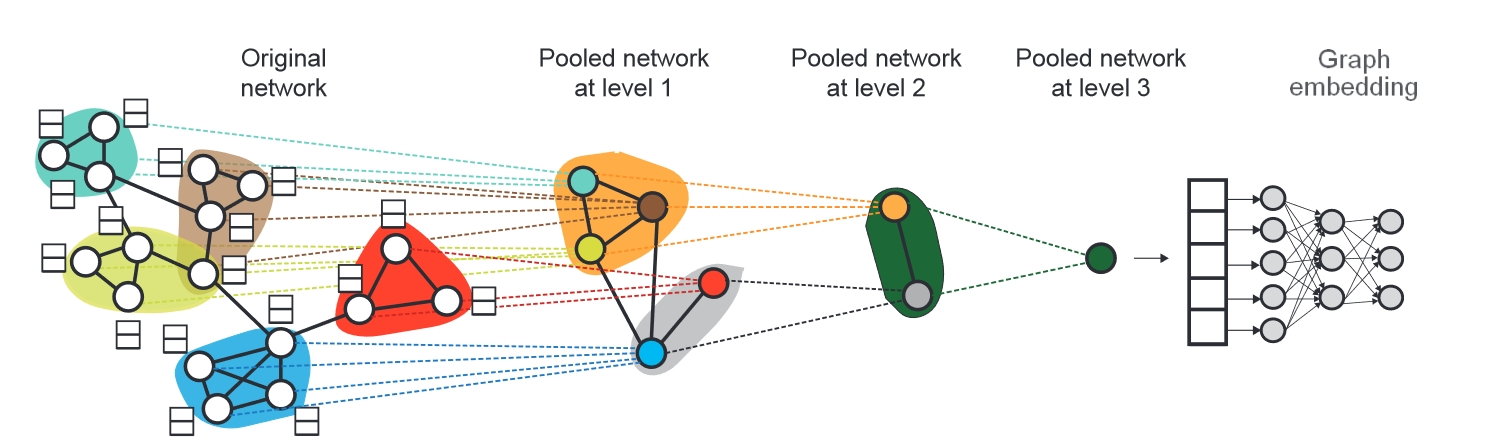
\includegraphics[width=0.5\textwidth]{figures/diffpool.jpg}
        \caption{Illustration of the DiffPool method taken from \cite{ying-2018}. The last feedforward neural network is used to obtain the graph embedding.}
        \label{fig:diffpool}
    \end{figure}
    Ying et al. have also shown in [Proposition 1, \cite{ying-2018}] that the permutation invariance of the DiffPool method is guaranteed, which is a crucial property for graph embedding methods.
    \subsection{Language modelling}

    We used a pretrained large language model (LLM) to encode the text. Specifically, we settled on \texttt{sentence-transformers/all-MiniLM-L6-v2} which is a distilled version of MiniLM \cite{wang-2020} known for its efficiency and relatively small size. The sentence embeddings are obtained by averaging the embeddings of the tokens in the sentence, which yields a 384-dimensional vector.

    \section{Training}

    \subsection{Model Evolution throughout the Challenge}
    Throughout the challenge, we tried different models and training procedures. We started with a slightly modified version of the baseline method with a "distlibert" language Transformer model trained by distilling BERT base, and ended up, for the final submission, with an ensemble of XX models. We recap in the following table the big landmarks of our model evolution.

    \begin{table}[H]
        \centering
        \begin{tabular}{c|c|c|c|c}
            \toprule
            \textbf{N°} & \textbf{Text Encoder} & \textbf{Graph Encoder} & \textbf{Main characteristics} & \textbf{Score} \\
            \midrule
            1 & DistilBERT & GAT & Baseline & 0.5 \\
            2 & MiniLM & GAT & \specialcell[r]{3 GAT layers\\3 attention layers} & 0.74 \\
            3 & MiniLM & DiffPool & 2 layers
        \end{tabular}
        \caption{Model evolution throughout the challenge.}
    \end{table}

    \subsection{Loss Functions}

    \subsection{Training Procedure and implementation details}

    \subsection{Trained models' hyperparameters}

    \section{Results}

    \subsection{Results per trained model}
    \subsection{Global results after ensembling}
    \subsection{Execution time}

    \section{Other non-conclusive approaches}
    \subsection{PathNN}
    \subsection{Condorcet Fusion}
    \subsection{Alternate training procedure}

    \newpage

    \bibliography{bibliography}

\end{multicols}

\end{document}
